\documentclass[aspectratio=169]{beamer} 
\usepackage[T1]{fontenc}
\usepackage[utf8]{inputenc}
\usepackage{plex-sans}
\usepackage[scale=0.85]{plex-mono}
\usepackage{amsmath}
\usepackage{amssymb}
\usepackage[british]{babel}
\usepackage[backend=biber,style=apa,citetracker=true]{biblatex}
\usepackage{csquotes}
\usepackage{hyperref}
\usepackage[overlay, absolute]{textpos}
\usepackage{tikz}
\usepackage{array,multirow,graphicx}
\usepackage{booktabs}
\usepackage{subcaption}
\usepackage{transparent}
\usepackage{multicol}

% TikZ libraries for relative positioning and better looking arrows
\usetikzlibrary{positioning, arrows.meta}

% BibLaTeX sources
\addbibresource{literature.bib}

% Urls the same color as text
\urlstyle{same}

% Use numbers instead of icons in the bibliography
\setbeamertemplate{bibliography item}[text]

% B&W color theme
\usecolortheme{seagull}

% Use symbols instead of numbers for footnotes
% \renewcommand{\thefootnote}{\fnsymbol{footnote}}

% don't show Beamer buttons
\beamertemplatenavigationsymbolsempty

% more spacing below footnotes
\setbeamertemplate{footline}{\vspace{6.7pt}}

% make captions numbered (beamer by default uses Figure: caption instead of Figure 1: caption)
\setbeamertemplate{caption}[numbered]

%Information to be included in the title page:
\title{Tools for Gossip} 
\subtitle{Bachelor's Project} 
\author{%
    R.A. Meffert\\\vspace{5pt}
    {\small Supervisor: Dr. B.R.M Gattinger} 
} 
\institute{University of Groningen} 
\date{Bachelor's Symposium, January 25, 2021}

\begin{document}
{\setbeamertemplate{background}
{\transparent{0.2}\includegraphics[width=\paperwidth,keepaspectratio]{images/phone.jpg}}
\frame{\titlepage}
}
\begin{frame}[c]{About this bachelor's project}
    \begin{multicols}{2}
        \begin{itemize}
            \item<1-> The telephone problem \only<1->{\footcite[e.g.][]{tijdeman_telephone_1971}}
            \item<2-> Dynamic gossip \only<2->{\footcite{van_ditmarsch_dynamic_2018}}
            \item<3-> Goal: easy-to-use educational tool
        \end{itemize}
        \columnbreak
        \begin{figure}
            \includegraphics[width=\linewidth]{images/agents.jpg}
            \caption{Two agents merging their secrets}
        \end{figure}
    \end{multicols}
    \begin{textblock*}{.5\paperwidth}[1,1](.99\paperwidth,.98\paperheight)
            \hfill \tiny\textcolor{gray!50}{Image credit: people photo created by shurkin\_son - www.freepik.com}
    \end{textblock*}
\end{frame}
%--- Next Frame ---%
\begin{frame}[c]{Why dynamic gossip?}
    \begin{figure}
      \begin{subfigure}[t]{.3\paperwidth}
        \centering
        \includegraphics[height=.3\paperheight]{images/bitcoin.png}
        \caption*{Blockchain}
      \end{subfigure}
      \qquad
      \begin{subfigure}[t]{.3\paperwidth}
        \centering
        \includegraphics[height=.3\paperheight]{images/ssbc.png}
        \caption*{Social Media}
      \end{subfigure}

      \bigskip

      \begin{subfigure}[t]{.3\paperwidth}
        \centering
        \includegraphics[height=.3\paperheight]{images/dna.png}
        \caption*{Genome analysis}
      \end{subfigure}
      \qquad
      \begin{subfigure}[t]{.3\paperwidth}
        \centering
        
\includegraphics[height=.3\paperheight]{images/network.pdf}
        \caption*{Distributed databases}
      \end{subfigure}
    \end{figure}
\end{frame}
%--- Next Frame ---%
\begin{frame}[c]{Example}
    \centering
    \vspace{1cm}
    
    \resizebox {.7\textwidth} {!} {
        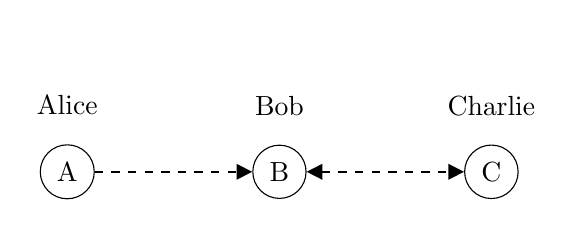
\begin{tikzpicture}[node distance=2cm]
            \node [draw, circle] (A) {A};
            \node [draw, circle, right=of A] (B) {B};
            \node [draw, circle, right=of B] (C) {C};
        
            \node [above=.25cm of A] (AName) {Alice};
            \node [above=.25cm of B] (BName) {Bob};
            \node [above=.25cm of C] (CName) {Charlie};
            
            % white text to keep spacing the same
            \node [above=1cm of B, text=white] (BName) {After call none};
        
            \draw [dashed, thick, -{Triangle[length=2mm]}] 
                (A) -- (B);
            \draw [dashed, thick, {Triangle[length=2mm]}-{Triangle[length=2mm]}] 
                (B) -- (C);
        \end{tikzpicture}
    }
    \begin{align*}
        N &= \{ (a, b), (b, c), (c, b) \} \\
        S &= I_A
    \end{align*}
\end{frame}
%--- Next Frame ---% 
\begin{frame}[c]{Example}
    \centering
    \vspace{1cm}
    
    \resizebox {.7\textwidth} {!} {
        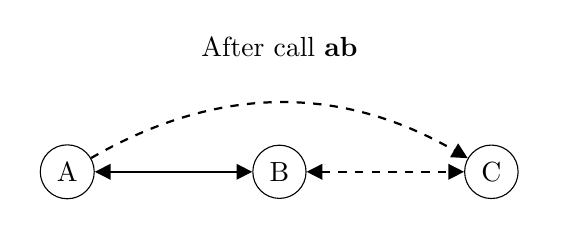
\begin{tikzpicture}[node distance=2cm]
            \node [draw, circle] (A) {A};
            \node [draw, circle, right=of A] (B) {B};
            \node [draw, circle, right=of B] (C) {C};
        
            % white text to keep spacing the same
            \node [above=.25cm of A, text=white] (AName) {Alice};
            \node [above=.25cm of B, text=white] (BName) {Bob};
            \node [above=.25cm of C, text=white] (CName) {Charlie};
            
            \node [above=1cm of B] (BName) {After call \textbf{ab}};
        
            \draw [solid, thick, {Triangle[length=2mm]}-{Triangle[length=2mm]}] 
                (A) -- (B);
            \draw [dashed, thick, -{Triangle[length=2mm]}] 
                (A) to[bend left] (C);
            \draw [dashed, thick, {Triangle[length=2mm]}-{Triangle[length=2mm]}] 
                (B) -- (C);

        \end{tikzpicture}
    }
    \begin{align*}
        N &= I_A \cup \{ (a, b), (a, c), (b, a), (b, c), (c, b) \} \\
        S &= I_A \cup \{ (a, b), (b, a) \}
    \end{align*}
\end{frame}
%--- Next Frame ---%
\begin{frame}[c]{Example}
    \centering
    \vspace{1cm}
    
    \resizebox {.7\textwidth} {!} {
        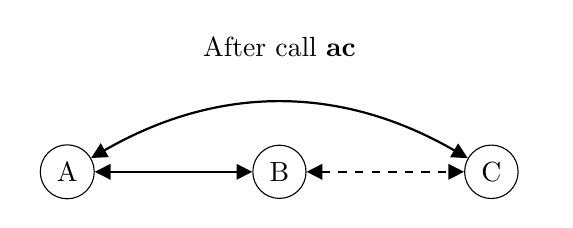
\begin{tikzpicture}[node distance=2cm]
            \node [draw, circle] (A) {A};
            \node [draw, circle, right=of A] (B) {B};
            \node [draw, circle, right=of B] (C) {C};
    
            % white text to keep spacing the same
            \node [above=.25cm of A, text=white] (AName) {Alice};
            \node [above=.25cm of B, text=white] (BName) {Bob};
            \node [above=.25cm of C, text=white] (CName) {Charlie};
            
            \node [above=1cm of B] (BName) {After call \textbf{ac}};
        
            \draw [solid, thick, {Triangle[length=2mm]}-{Triangle[length=2mm]}] 
                (A) -- (B);
            \draw [solid, thick, {Triangle[length=2mm]}-{Triangle[length=2mm]}] 
                (A) to[bend left] (C);
            \draw [dashed, thick, {Triangle[length=2mm]}-{Triangle[length=2mm]}] 
                (B) -- (C);

        \end{tikzpicture}
    }
    \begin{align*}
        N &= A^2 \\
        S &= I_A \cup \{ (a, b), (a, c), (b, a), (c, a)\}
    \end{align*}
\end{frame}
%--- Next Frame ---%
\begin{frame}[c]{Example}
    \centering
    \vspace{1cm}

    \resizebox {.7\textwidth} {!} {
        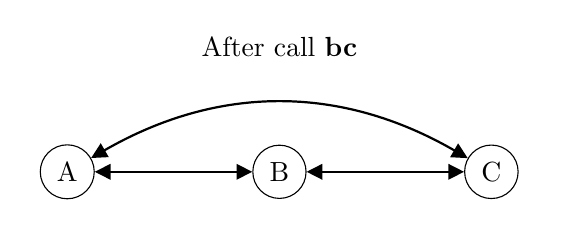
\begin{tikzpicture}[node distance=2cm]
            \node [draw, circle] (A) {A};
            \node [draw, circle, right=of A] (B) {B};
            \node [draw, circle, right=of B] (C) {C};
    
            % white text to keep spacing the same
            \node [above=.25cm of A, text=white] (AName) {Alice};
            \node [above=.25cm of B, text=white] (BName) {Bob};
            \node [above=.25cm of C, text=white] (CName) {Charlie};
            
            \node [above=1cm of B] (BName) {After call \textbf{bc}};
        
            \draw [solid, thick, {Triangle[length=2mm]}-{Triangle[length=2mm]}] 
                (A) -- (B);
            \draw [solid, thick, {Triangle[length=2mm]}-{Triangle[length=2mm]}] 
                (A) to[bend left] (C);
            \draw [solid, thick, {Triangle[length=2mm]}-{Triangle[length=2mm]}] 
                (B) -- (C);

        \end{tikzpicture}
    }
    \begin{align*}
        N &= A^2 \\
        S &= A^2
    \end{align*}
\end{frame}
%--- Next Frame ---%
\begin{frame}[t]{The tool}
    \includegraphics[width=\linewidth]{images/tool.png}
\end{frame}
%--- Next Frame ---%
\begin{frame}[t]{Graph visualisation}
    \includegraphics[width=\linewidth]{images/tool-graph.png}
\end{frame}
%--- Next Frame ---%
\begin{frame}[t]{Gossip protocols}
    \includegraphics[width=\linewidth]{images/tool-protocol.png}
\end{frame}
%--- Next Frame ---%
\begin{frame}[t]{Call sequence validation \& execution}
    \includegraphics[width=\linewidth]{images/tool-sequence.png}
\end{frame}
%--- Next Frame ---%
\begin{frame}[t]{Execution tree}
    \includegraphics[width=\linewidth]{images/tool-history.png}
\end{frame}
%--- Next Frame ---%
\begin{frame}[c]{Implementation}
    \begin{multicols}{2}
        \begin{itemize}
            \item<1-> Language: Elm \footcite{czaplicki_asynchronous_2013}
            \begin{itemize}
                \item Open source, functional web language
            \end{itemize}
            \item<2-> Pure functions
            \begin{itemize}
                \item Easier to translate mathematical functions into code
            \end{itemize}
            \item<3-> Compiled to Javascript
            \begin{itemize}
                \item Free cross-platform compatibility
            \end{itemize}
            \item<4-> Static type checking
            \begin{itemize}
                \item Zero runtime exceptions
            \end{itemize}
        \end{itemize}
        \columnbreak
        \begin{figure}
            \centering
            
\includegraphics[width=.5\linewidth]{images/Elm_logo.pdf}
        \end{figure}
    \end{multicols}
\end{frame}
%--- Next Frame ---%
\begin{frame}[c]{Survey}
    \begin{multicols}{2}
        \begin{itemize}
            \item<1-> Short exploratory survey
            \item<2-> 12 respondents
            \item<3-> General impression: positive
            \item<4-> Useful feedback
        \end{itemize}
        \columnbreak
        \begin{figure}
            \centering
            \includegraphics[width=\linewidth]{images/survey.jpg}
        \end{figure}
    \end{multicols}
\end{frame}
%--- Next Frame ---%
\begin{frame}[c]{Survey results}
    \begin{figure}
        \centering
        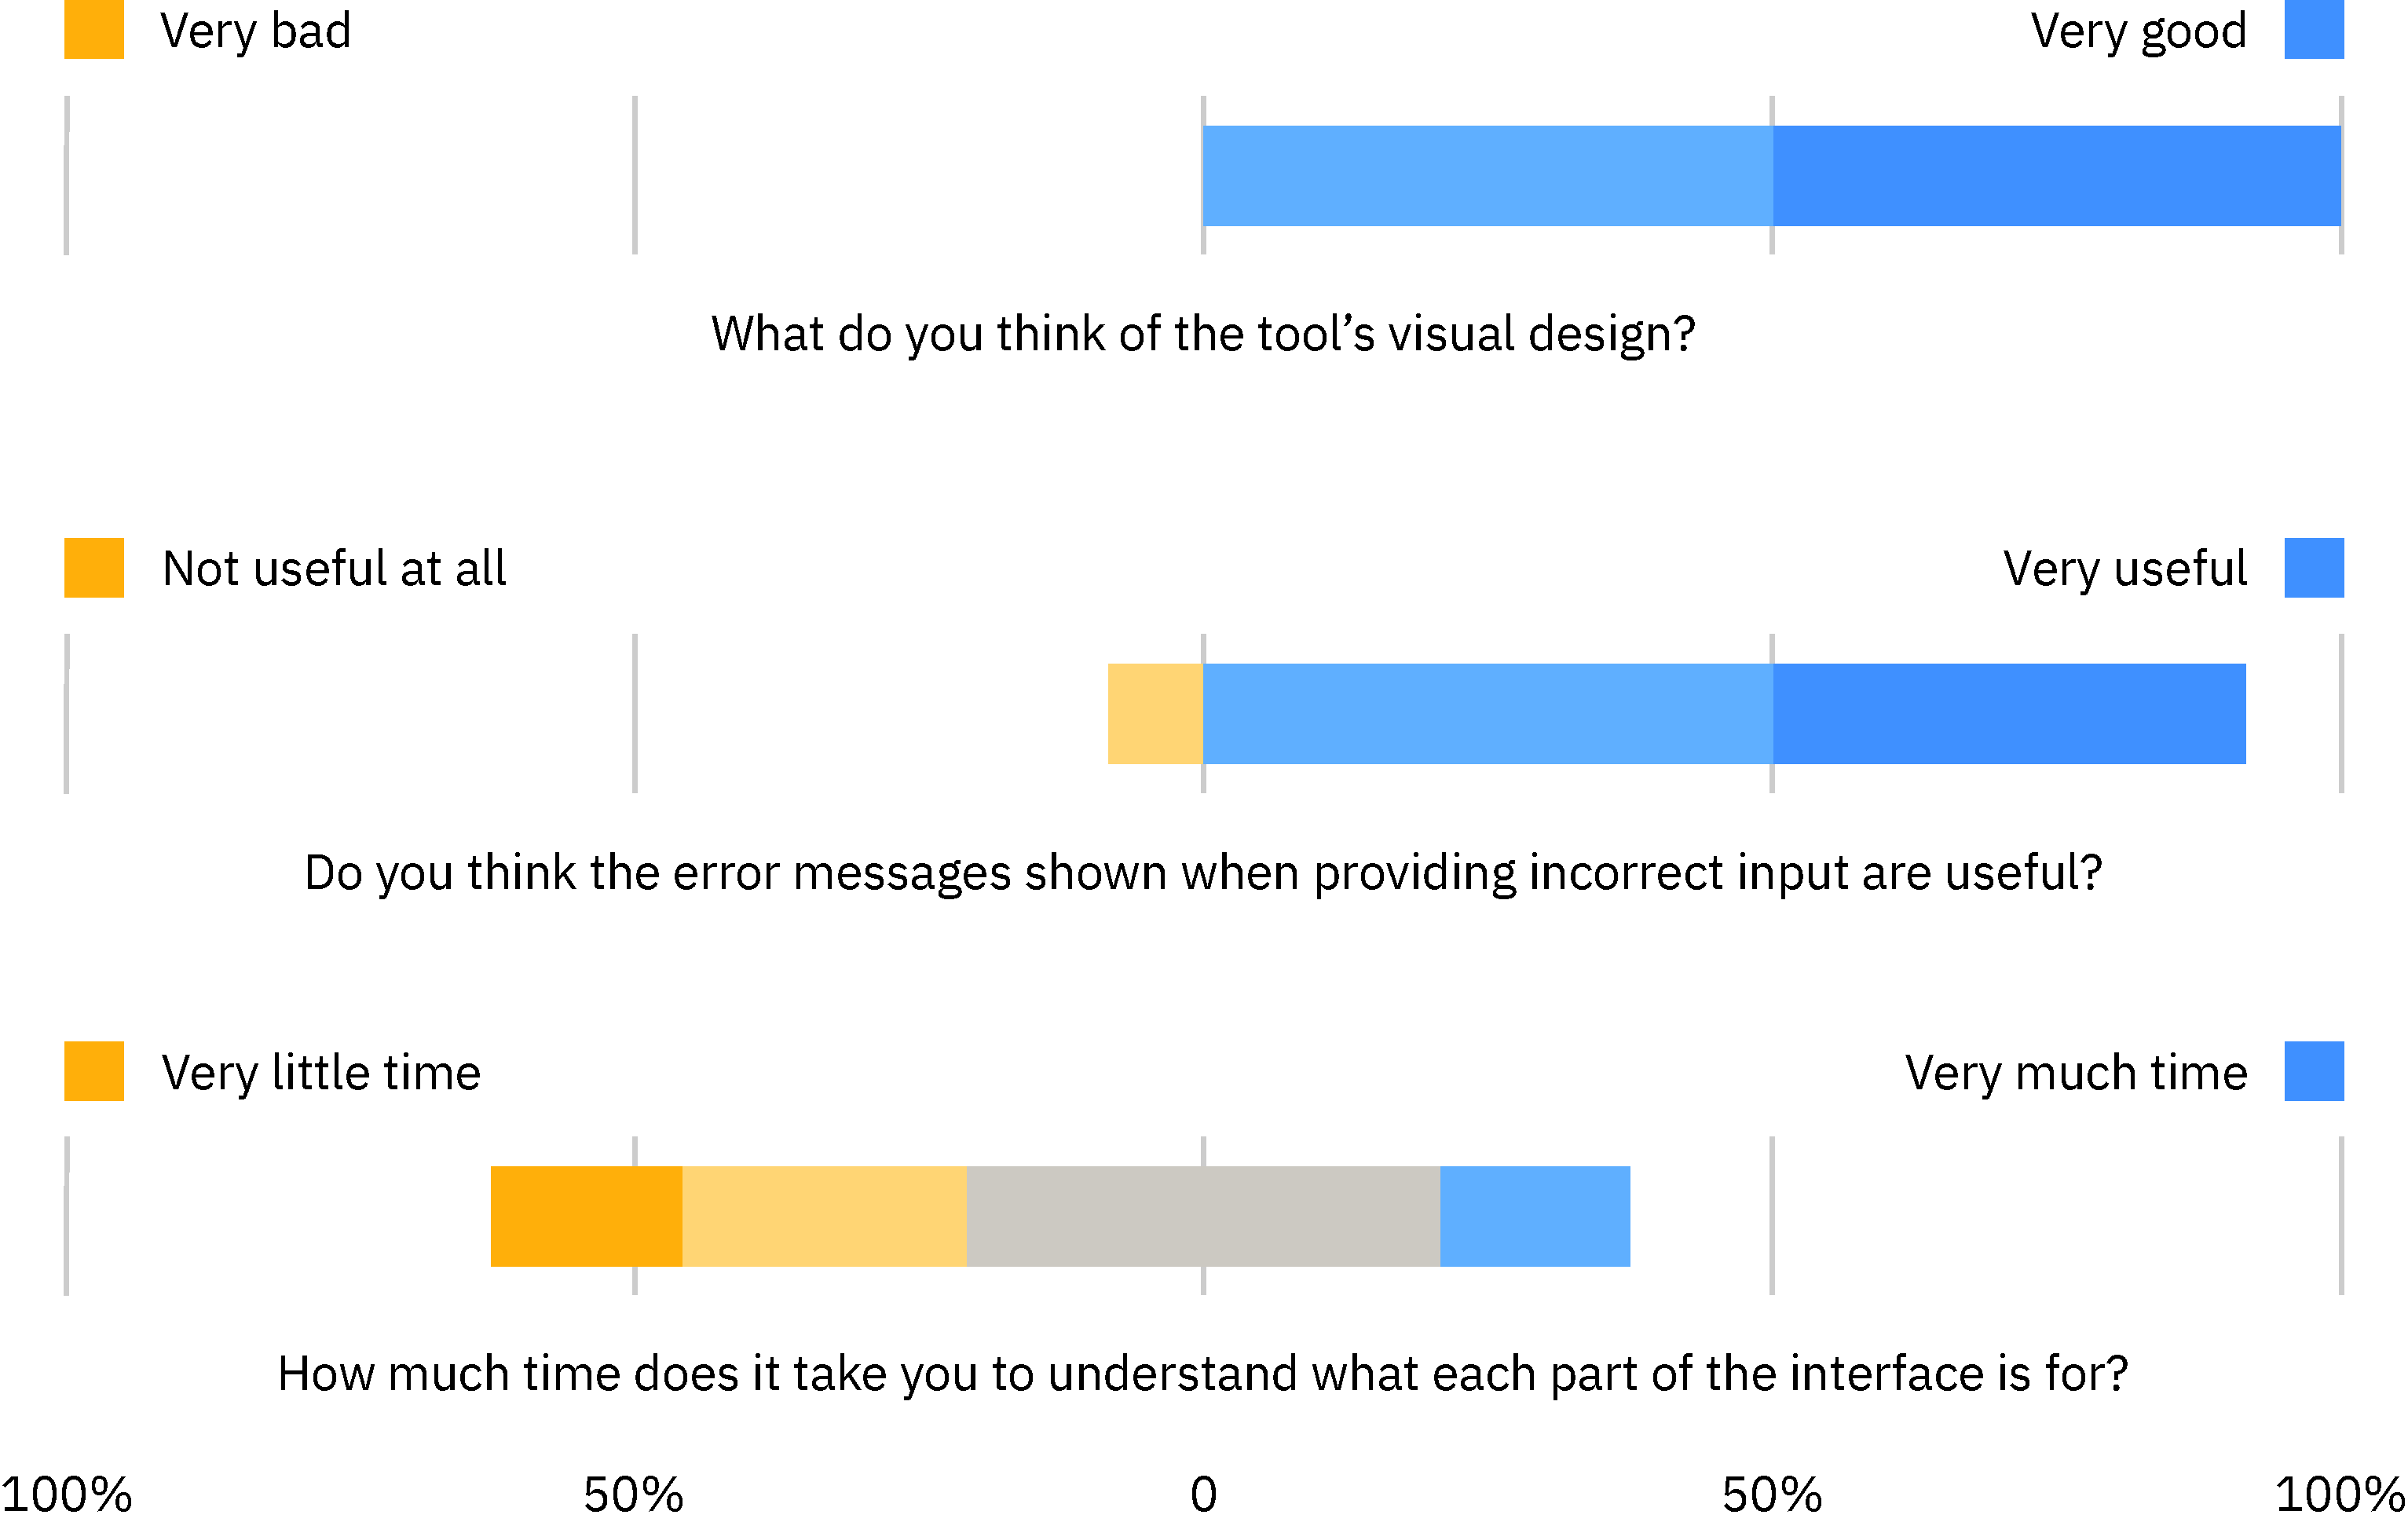
\includegraphics[width=.8\linewidth]{images/survey-likert.pdf}
    \end{figure}
\end{frame}
%--- Next Frame ---%
\begin{frame}[c]{Survey results}
    \begin{figure}
        \begin{subfigure}{.4\paperwidth}
            \centering
            
\includegraphics[width=.7\linewidth]{images/survey-study.pdf}
            \bigskip
            \caption*{\centering Do you think this tool could be useful in a study setting?}
        \end{subfigure}
        \hfill
        \begin{subfigure}{.4\paperwidth}
            \centering
            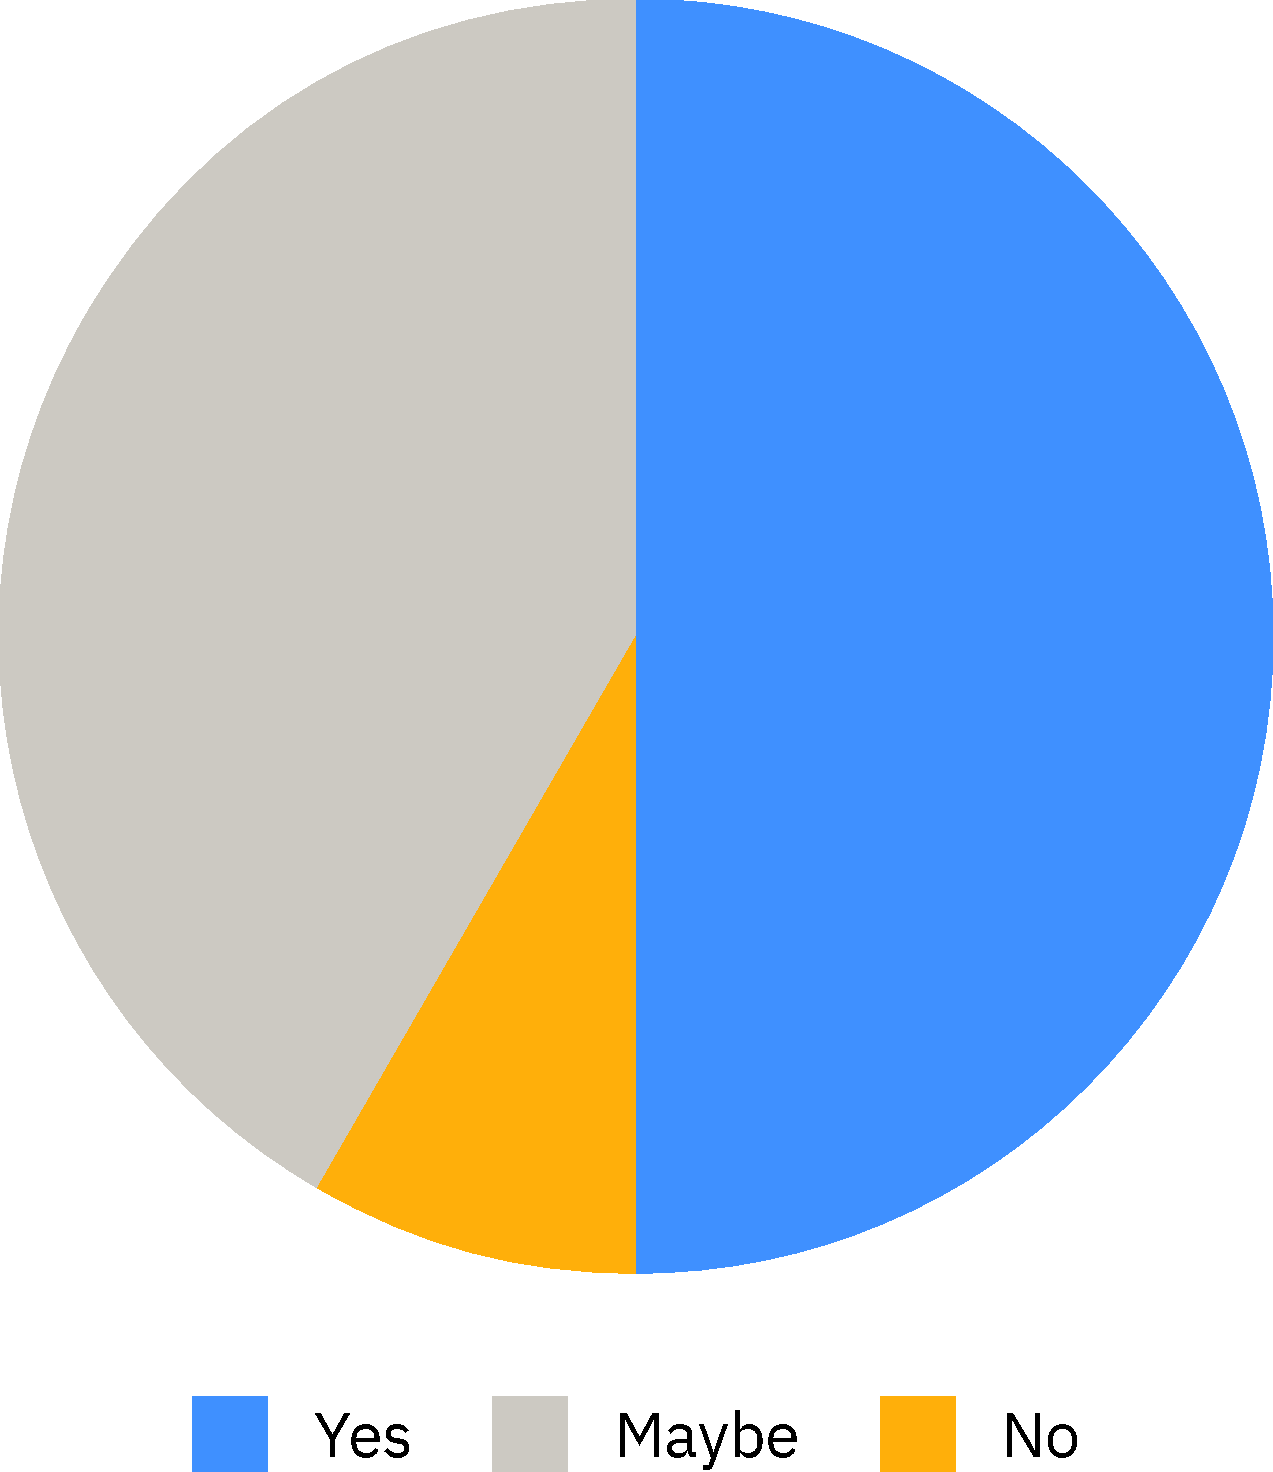
\includegraphics[width=.7\linewidth]{images/survey-research.pdf}
            \bigskip
            \caption*{\centering Do you think this tool could be useful in a research setting?}
        \end{subfigure}
    \end{figure}
\end{frame}
%--- Next Frame ---%
\begin{frame}[c]{Further research and extensions}
    \begin{multicols}{2}
        \begin{itemize}
            \item<1-> Unreliable gossip \footcite{martins_dealing_2020}
            \item<2-> Higher level knowledge \footcite{herzig_how_2017}
            \item<3-> Temporal gossip \footcite{slavkovik_temporal_2019}
            \item<4-> And more!
        \end{itemize}
        \columnbreak
        \begin{figure}
            \centering
            \includegraphics[width=\linewidth]{images/sattelite.jpg}
        \end{figure}
    \end{multicols}
\end{frame}
%--- Next Frame ---%
\begin{frame}[c]{Summary}
    \begin{multicols}{2}
        \begin{itemize}
            \item Tool for exploring dynamic gossip
            \begin{itemize}
                \item Graph visualisation
                \item Gossip protocols
                \item Call (sequence) evaluation \& execution
                \item Execution tree
            \end{itemize}
            \item Positively evaluated
            \item Open source + free license (GPLv3)
        \end{itemize}
        \columnbreak
        \begin{figure}
            \centering
            \includegraphics[width=.55\linewidth]{images/graph.png}
        \end{figure}
    \end{multicols}
\end{frame}
\begin{frame}[c]{Quick links}
    \begin{center}
        \begin{tabular}{rll}
                                    & \multicolumn{1}{c}{\scriptsize RESULT}                                & \multicolumn{1}{c}{\scriptsize SOURCE CODE}\vspace{5pt}\\
            {\scriptsize TOOL}      & \href{https://r3n.nl/bsc/gossip}{\textcolor{gray}{r3n.nl/bsc}/gossip} & \href{https://r3n.nl/bsc/src/gossip}{\textcolor{gray}{r3n.nl/bsc}/src/gossip}\vspace{5pt}\\
            {\scriptsize THESIS}    & \href{https://r3n.nl/bsc/thesis}{\textcolor{gray}{r3n.nl/bsc}/thesis} & \href{https://r3n.nl/bsc/src/thesis}{\textcolor{gray}{r3n.nl/bsc}/src/thesis}\vspace{5pt}\\
            {\scriptsize SLIDES}    & \href{https://r3n.nl/bsc/slides}{\textcolor{gray}{r3n.nl/bsc}/slides} & \href{https://r3n.nl/bsc/src/slides}{\textcolor{gray}{r3n.nl/bsc}/src/slides}
         \end{tabular}
          
         \bigskip
          
         \textcolor{gray}{\tiny Thesis will be available after Februari 1st, slides after today}
    \end{center}
\end{frame}
%--- Next Frame ---%
\begin{frame}[t,allowframebreaks]
    \frametitle{References}
    \printbibliography
\end{frame}

\end{document}
